\documentclass[a4paper, 11pt]{article}
\usepackage{geometry}
\geometry{letterpaper, margin=1in}
\usepackage{amsmath}
\usepackage{amssymb}  
\usepackage{amsthm}
\usepackage{ulem} 
\usepackage{graphicx}
\usepackage{cancel} 
\usepackage{enumitem} 
\graphicspath{ {images/} }


\newtheorem*{theorem}{Theorem}

\begin{document}
%Header-Make sure you update this information!!!!
\noindent
\large\textbf{Thermal Physics - PH441} \hfill \textbf{John Waczak} \\
\normalsize Day 17 \hfill  Date: \today \\

\subsection*{Fermion-Statistics}
	Recall from last class, we discussed how we could take the many bodied wave function $\Psi(\vec{r}_1, \vec{r}_2, ...\vec{r}_n) = $ slater determinant that ensures that we have the correct anti-symmetric combination of orbitals. These orbitals $\phi_i(\vec{r}_j)$ are the energy eigenstates of the single particle system. The \textit{trick} we are going to be using is to take each of the orbitals and treat them as if they were a separate systems... weird. \\ 
	
	\noindent Now think of our $\phi_i(\vec{r})$ as having an occupancy of 1 or 0.\\
	
	
	\begin{figure}[!hbt]
		\centering 
		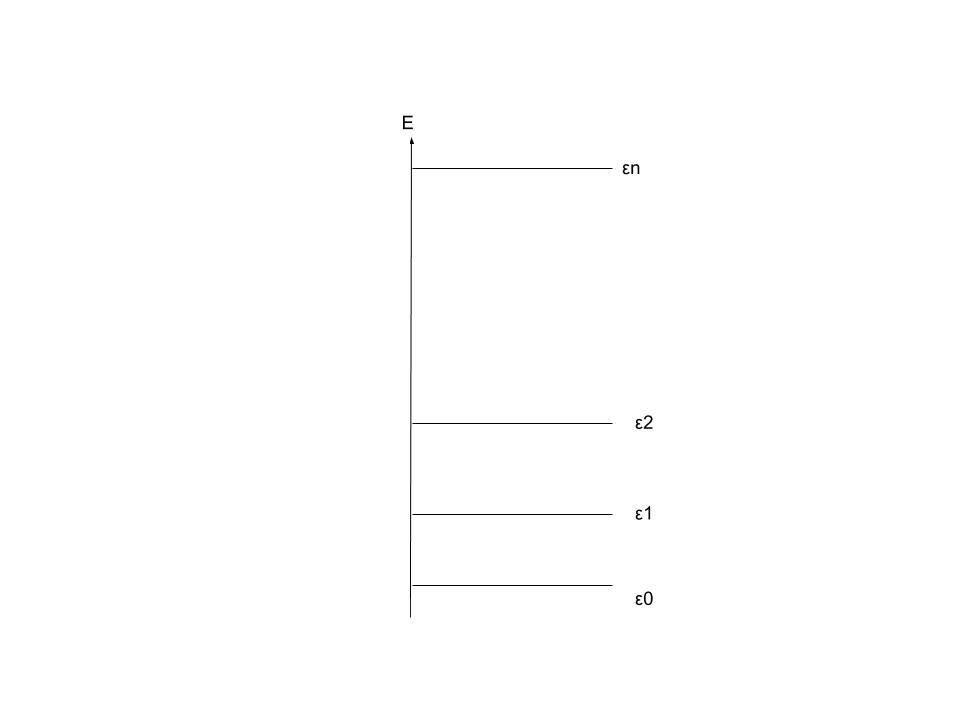
\includegraphics[width=0.6\columnwidth]{energyLevels}
		\caption{general idea of energy levels four our single particle} 
	\end{figure}
	
	
	 We have that our Gibbs sum for a $\phi_i$ From Puali's exclusion principle, we can only have one particle : 
		\begin{align*}
			\mathbb{Z} &= \sum_i e^{-\beta(E_i-\mu N_i)} \\ 
				&= 1 + e^{-\beta(\epsilon - \mu)} \\ 
			\Rightarrow \langle E \rangle &= \epsilon \frac{e^{-\beta(\epsilon-\mu)}}{1 + e^{-\beta(\epsilon - \mu)}} \\ 
			&= \epsilon\frac{1}{1+ e^{\beta(\epsilon - \mu)}} \\
			\langle N \rangle &=  \frac{e^{-\beta(\epsilon-\mu)}}{1 + e^{-\beta(\epsilon - \mu)}} \\
				&= \frac{1}{1+ e^{\beta(\epsilon - \mu)}}  = \text{Fermi-Dirac function} 
		\end{align*}
	
	\noindent \textbf{Definitions} The \textit{Fermi-Level} is synonymous with the chemical potential $\mu$. The \textit{Fermi-energy} is $\mu(T=0)$. 
	
	
\subsection*{Boson-statistics}
	We do not have the anti-symmetry requirement and so we can have many combinations of orbitals to make a combined state. Now our orbitals $\phi_i$ with energy $\epsilon$ and occupancy $N = 0, 1, 2, 3,... \infty$. 
		\begin{align*}
			\mathbb{Z} &= 1+\sum_{j=1}^\infty \Big(e^{-\beta(\epsilon j-\mu j)}\Big)\\
				&= 1+\sum_{j=1}^\infty \Big(e^{-\beta(\epsilon -\mu )}\Big)^j \\ 
				&= \frac{1}{1-e^{-\beta(\epsilon-\mu)}}\\
			\langle N \rangle &= \sum_j\frac{j e^{-\beta(\epsilon-\mu)j}}{\mathbb{Z}} \\
				&= \frac{1}{\mathbb{Z}}\frac{\partial\mathbb{Z}}{\partial(\mu \beta)} \\ 
				&= \frac{e^{-\beta(\epsilon-\mu)}}{1-e^{-\beta(\epsilon-\mu)}} = \frac{1}{e^{\beta(\epsilon-\mu)}-1} = f_{BE}(\epsilon)
		\end{align*}
	
	
	
	
	
	
	
\end{document}



























